\subsection{Collegamento Nodi al Flusso Dati}\label{Collegamento}

L'operazione di collegamento dei nodi della rete bayesiana al flusso dati è probabilmente la più articolata e dispendiosa del prodotto realizzato. Al fine di fornirne una spiegazione esaustiva ma al contempo intuitiva tale operazione verrà suddivisa in svariati passaggi:
~\\

\textbf{PREAMBOLO:} L'utente, a seguito del caricamento di una rete bayesiana (§\ref{ReteB}), visualizza la lista dei nodi di cui tale rete è costituita, tale situazione è presentata in Figura \ref{NodiRete}. Oltre al nominativo del nodo stesso viene visualizzata una checkbox che indica se il nodo in questione sia o meno collegato ad un flusso dati. Nel caso di nodo collegato viene visualizzato anche un pulsante \textbf{Scollega} attraverso cui è possibile scollegare il nodo dal flusso dati con un unico click.\\
Della lista di nodi visualizzata l'utente ha la possibilità di collegare ogni nodo, senza eccezioni, ad un flusso dati desiderato.
~\\

\textbf{PASSAGGIO 1:} L'utente clicca il nominativo del nodo che desidera collegare per accedere al \textbf{Pannello di Collegamento} (Figura \ref{PannelloNodo}), ove può configurare le necessarie impostazioni di collegamento per il nodo in esame.

\begin{figure}[H]
	\begin{center}
		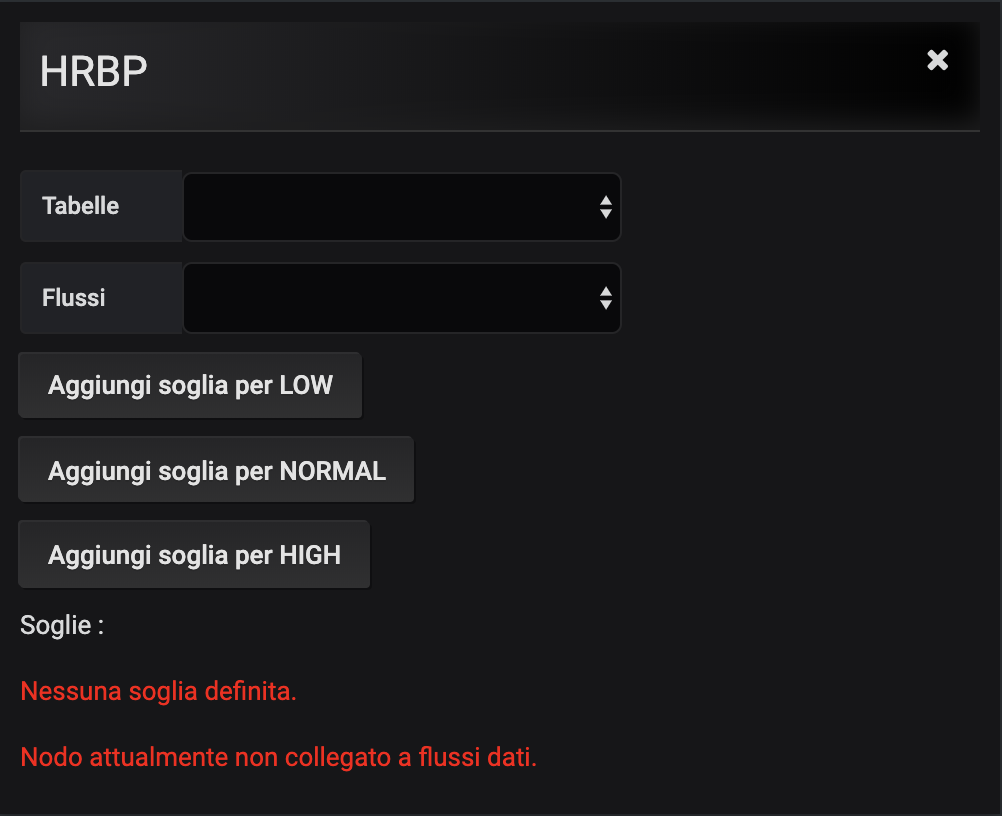
\includegraphics[scale=0.6]{./images/PannelloNodo.png}
		 \caption{Pannello di Collegamento del Nodo}	
		 \label{PannelloNodo}
	\end{center}
\end{figure}

\pagebreak

\textbf{PASSAGGIO 2:} Le prime impostazioni che l'utente è invitato a configurare riguardano la scelta della tabella, e del conseguente flusso dati (Figura \ref{PannelloNodo}), del database (selezionato in §\ref{SelectDB}). Tali impostazioni determinano univocamente lo specifico flusso dati di monitoraggio a cui l'utente collega il nodo della rete bayesiana.
~\\

\textbf{PASSAGGIO 3:} A questo punto l'utente deve configurare le soglie associate ad ogni possibile stato del nodo in esame. Tali soglie verranno verificate in sede di monitoraggio per associare un valore di evidenza al nodo della rete bayesiana in un dato istante.Possiamo suddividere questo passaggio in ultreriori cinque passi:
\begin{enumerate}
	\item L'utente seleziona \textbf{Aggiungi soglia} (pulsante presente in Figura \ref{PannelloNodo}) per aggiungere una soglia allo stato del nodo associato. È possibile aggiungere più soglie allo stesso stato;
	\item L'utente indica il valore numerico della soglia che sta definendo attraverso l'apposito campo dati visibile in Figura \ref{PannelloSoglie};
	\item L'utente seleziona, tramite la casella a scelta multipla, un valore tra i possibili: "<","<=",">" o ">=", per indicare la tipologia di soglia che sta configurando (Figura \ref{PannelloSoglie});
	\item Se lo desidera l'utente può etichettare la soglia come "critica" attraverso l'apposita checkbox (Figura \ref{PannelloSoglie}). In tal caso la verifica di tale soglia verrà fatta a prescindere dalla politica temporale delezionata in §\ref{policy};
	\item Se lo desidera l'utente può rimuovere una soglia attraverso il pulsante \textbf{Remove} presente in Figura \ref{PannelloSoglie}.
\end{enumerate}

\begin{figure}[H]
	\begin{center}
		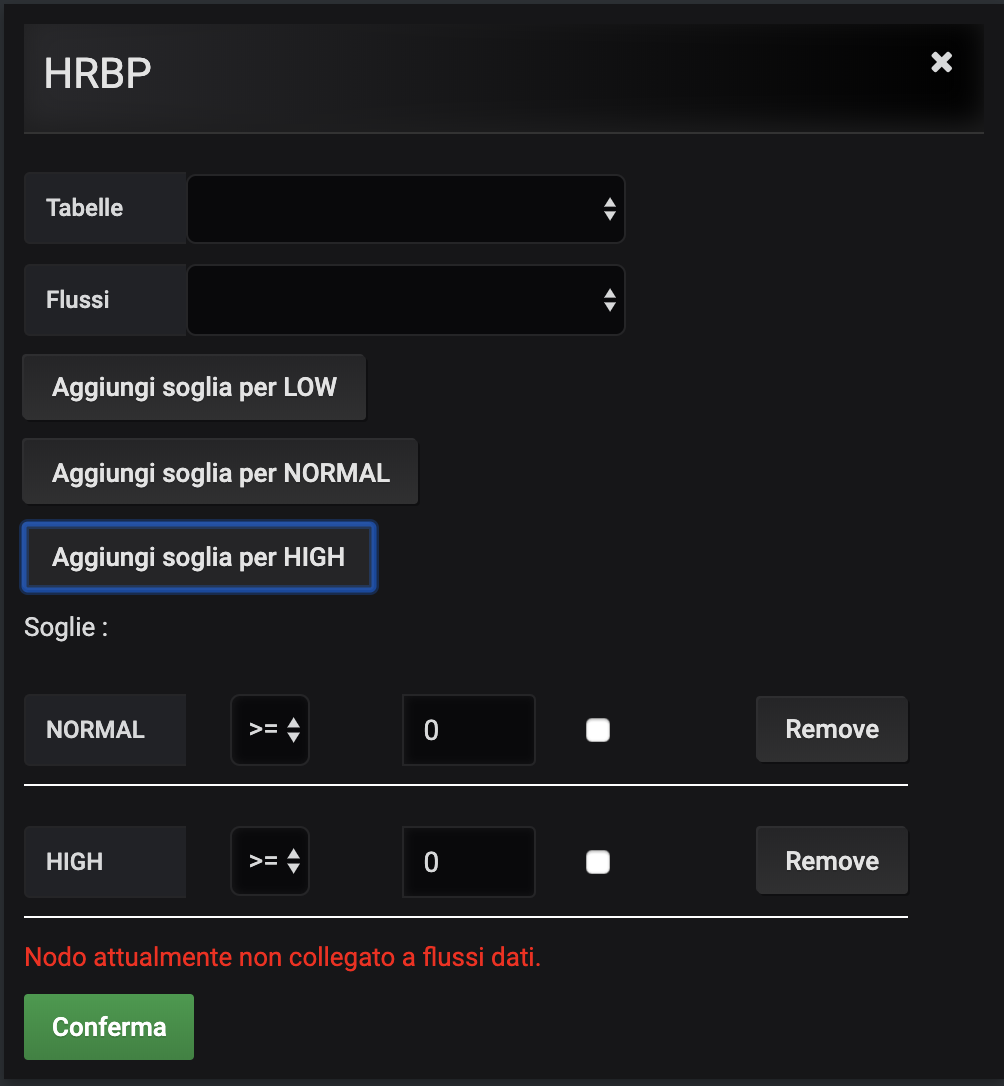
\includegraphics[scale=0.55]{./images/PannelloSoglie.png}
		 \caption{Pannello di Collegamento del Nodo con Vista sulla Definizione delle Soglie}	
		 \label{PannelloSoglie}
	\end{center}
\end{figure}

\textbf{PASSAGGIO 4:} Infine l'utente deve confermate le proprie scelte di collegamento del nodo attraverso il pulsante \textbf{Conferma} presente in Figura \ref{PannelloSoglie}.

~\\
A seguito del corretto collegamento del nodo al flusso dati l'utente verrà avvisato del buon esito dell'operazione da un messaggio di notifica (Figura \ref{NotificaCollegamento}).

\begin{figure}[H]
	\begin{center}
		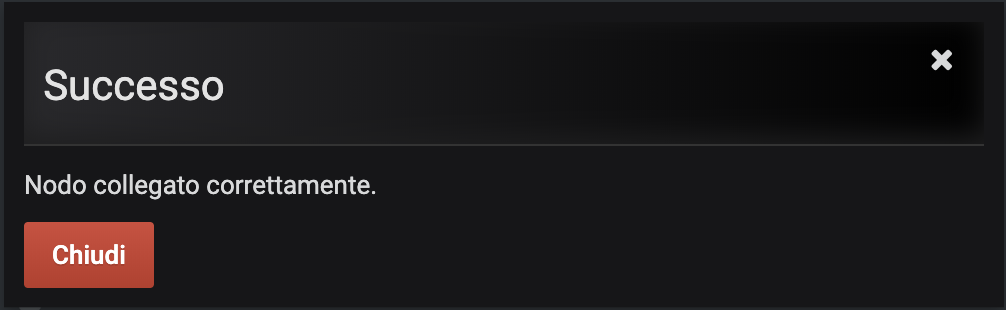
\includegraphics[scale=0.6]{./images/NotificaCollegamento.png}
		 \caption{Notifica di Avvenuto Collegamento del Nodo al Flusso Dati}	
		 \label{NotificaCollegamento}
	\end{center}
\end{figure}

L'utente visualizza inoltre, accanto al nodo in esame, la spunta sulla checkbox che ne indica lo stato di "Collegato al flusso dati" e il pulsante \textbf{Scollega Nodo} (Figura \ref{NodoCollegato}) per scollegare con un solo click il nodo al flusso dati.
 
 \begin{figure}[H]
	\begin{center}
		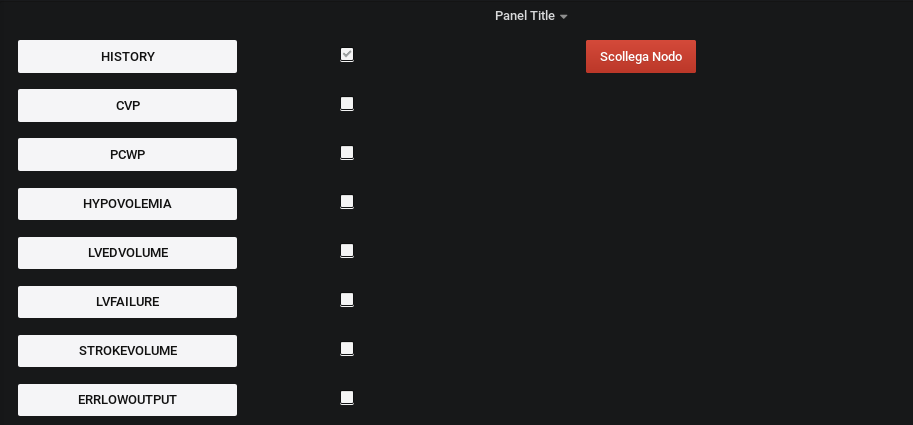
\includegraphics[scale=0.4]{./images/NodoCollegato.png}
		 \caption{Visualizzazione Nodo Collegato}	
		 \label{NodoCollegato}
	\end{center}
\end{figure}

\textbf{\textcolor{red}{ATTENZIONE}}: Nel caso in cui l'utente abbia commesso degli errori in fase di definizione delle impostazioni di collegamento l'operazione non va a buon fine e l'utente viene avvisato degli errori commessi da un messaggio di errore. Un esempio di tale situazione è fornito in Figura \ref{ErroreCollegamento}.

\begin{figure}[H]
	\begin{center}
		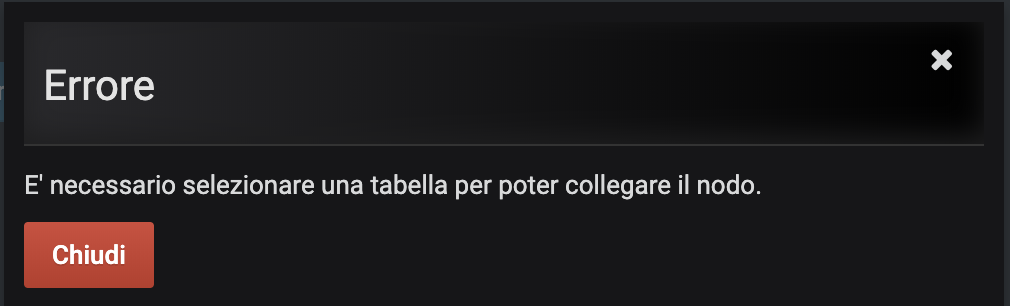
\includegraphics[scale=0.6]{./images/ErroreCollegamento.png}
		 \caption{Messaggio di Errore del Collegamento Nodo al Flusso Dati}	
		 \label{ErroreCollegamento}
	\end{center}
\end{figure}
 